\documentclass[11pt,t,usepdftitle=false,aspectratio=169]{beamer}

\usepackage{hyperref}
\usetheme[nototalframenumber,foot,logo]{uibk}


\title[Temperature Sensor]{ESP32 Temperature Sensor Project}
\subtitle{An IoT Implementation with Deep Sleep}
\author{Group 1}
\date{\today}

\begin{document}

\section{Introduction}

\begin{frame}
\frametitle{Prototype}
  \begin{figure}
    \centering
    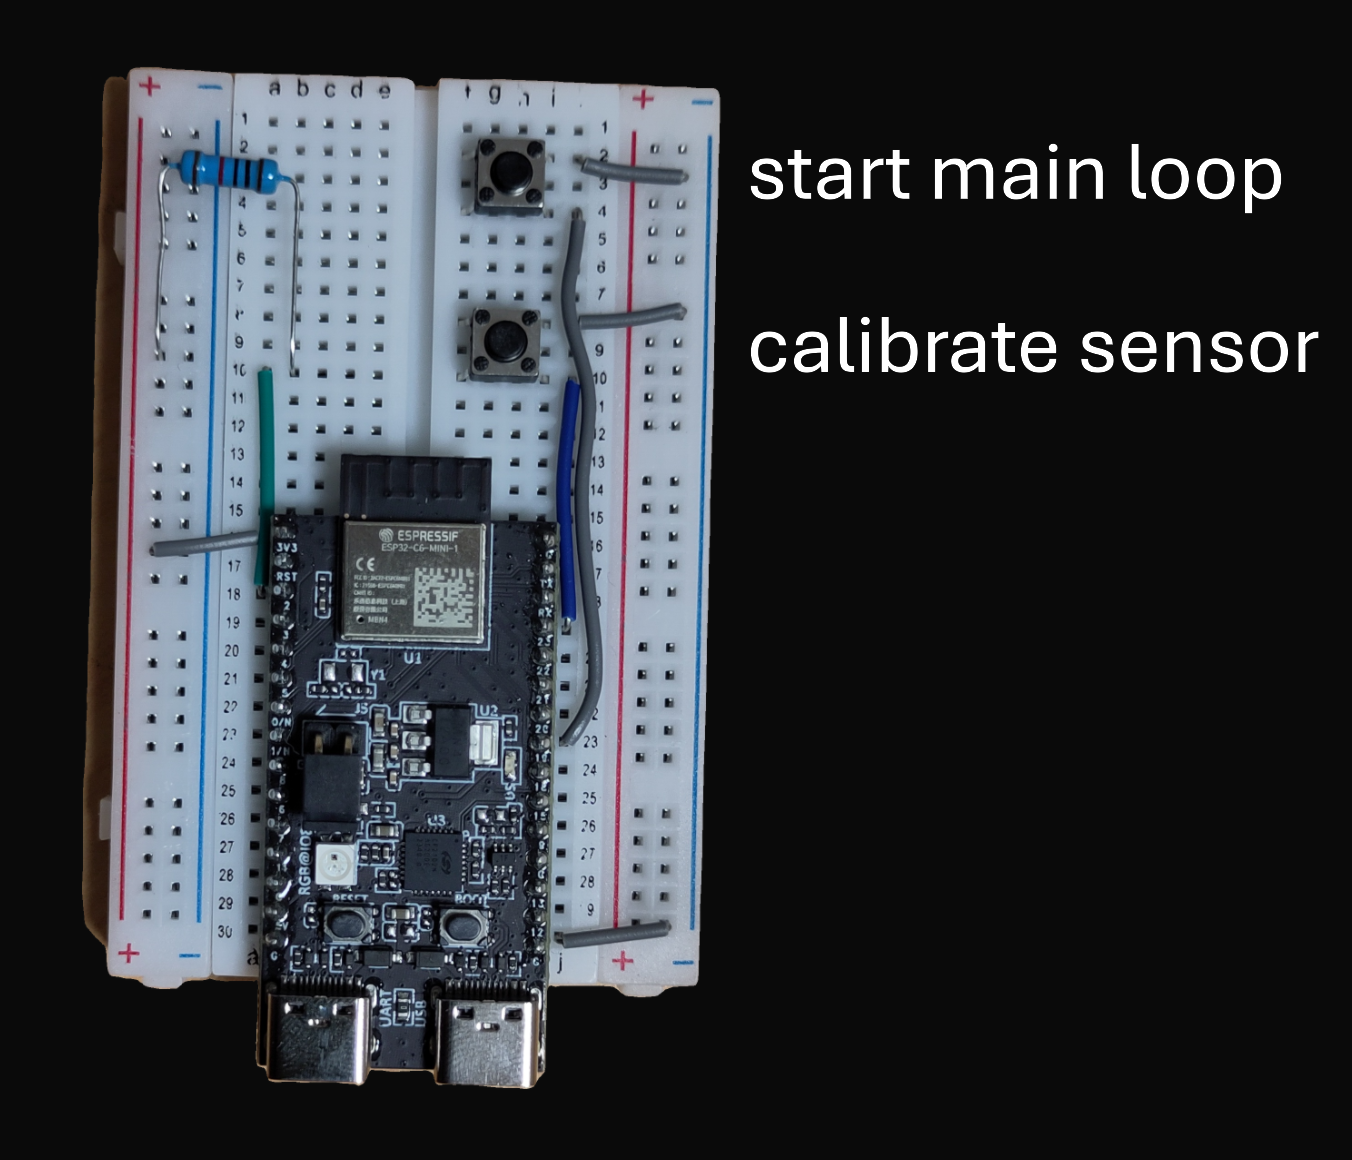
\includegraphics[width=0.5\textwidth]{_images/image_text.png}
  \end{figure}
\end{frame}


\begin{frame}
  \frametitle{Power Saving Features}
    \begin{itemize}
      \item Deep Sleep Mode
      \begin{itemize}
        \item 30 second sleep intervals between measurements
        \item 300 second sleep after 10 measurements completed
      \end{itemize}
      \item WiFi Power Optimization
      \begin{itemize}
        \item Modem sleep mode enabled
        \item Quick reconnect using stored WiFi config
        \item WiFi disabled during sleep
      \end{itemize}
      \item ADC Power Management
      \begin{itemize}
        \item One-shot ADC readings
        \item Only 5 samples per measurement
        \item ADC unit deleted before sleep
      \end{itemize}
    \end{itemize}
  \end{frame}


\begin{frame}
  \frametitle{Where is the thermistor?}
  \begin{figure}
    \centering
    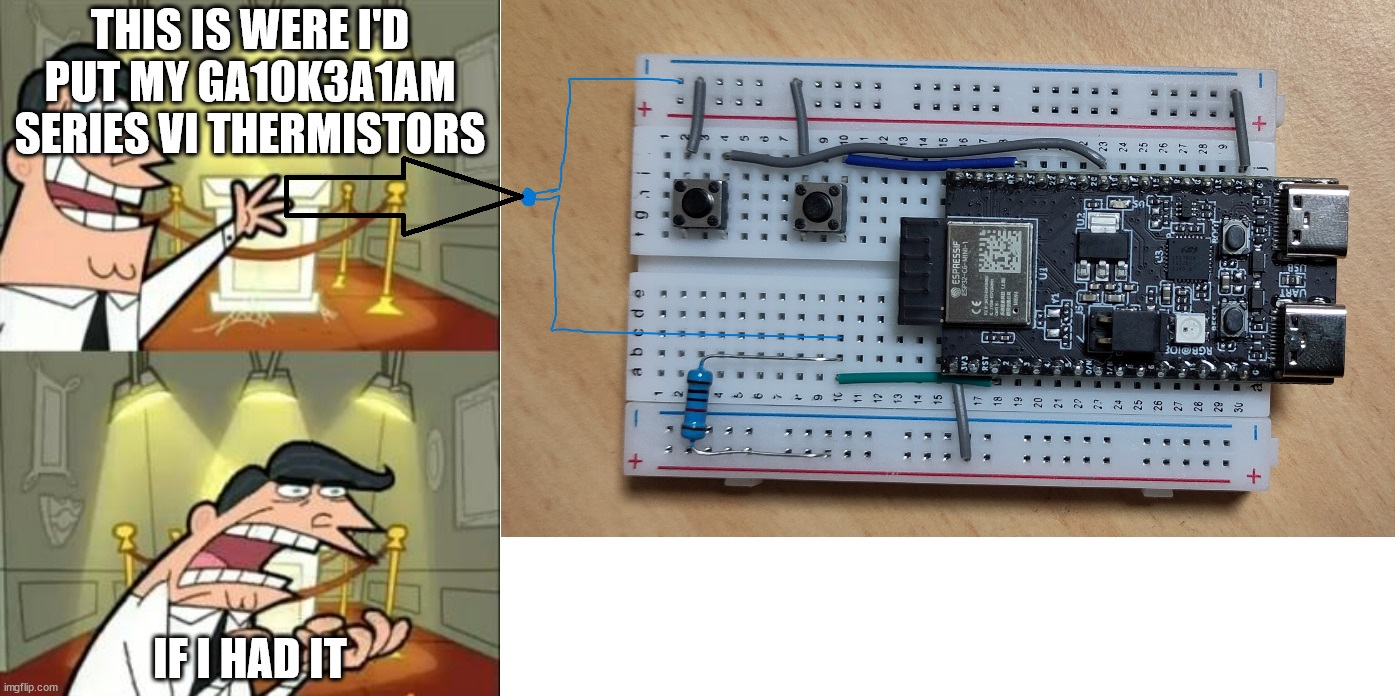
\includegraphics[width=0.8\textwidth]{_images/9i922u.jpg}
  \end{figure}
  Thank you for your attention!
\end{frame}


\end{document}

